\let\negmedspace\undefined
\let\negthickspace\undefined
\documentclass[journal]{IEEEtran}
\usepackage[a5paper, margin=10mm, onecolumn]{geometry}
%\usepackage{lmodern} % Ensure lmodern is loaded for pdflatex
\usepackage{tfrupee} % Include tfrupee package

\setlength{\headheight}{1cm} % Set the height of the header box
\setlength{\headsep}{0mm}     % Set the distance between the header box and the top of the text

\usepackage{gvv-book}
\usepackage{gvv}
\usepackage{cite}
\usepackage{amsmath,amssymb,amsfonts,amsthm}
\usepackage{algorithmic}
\usepackage{graphicx}
\usepackage{textcomp}
\usepackage{xcolor}
\usepackage{txfonts}
\usepackage{listings}
\usepackage{enumitem}
\usepackage{mathtools}
\usepackage{gensymb}
\usepackage{comment}
\usepackage[breaklinks=true]{hyperref}
\usepackage{tkz-euclide} 
% \usepackage{gvv}                                        
\def\inputGnumericTable{}                                 
\usepackage[latin1]{inputenc}                                
\usepackage{color}                                            
\usepackage{array}                                            
\usepackage{longtable}                                       
\usepackage{calc}                                             
\usepackage{multirow}                                         
\usepackage{hhline}                                           
\usepackage{ifthen}                                           
\usepackage{lscape}
\begin{document}

\bibliographystyle{IEEEtran}
\vspace{3cm}

\title{9.3.12-D}
\author{EE24BTECH11029 - J SHRETHAN REDDY}
\maketitle
% \newpage
% \bigskip
{\let\newpage\relax\maketitle}

\renewcommand{\thefigure}{\theenumi}
\renewcommand{\thetable}{\theenumi}
\setlength{\intextsep}{10pt} % Space between text and floats


\numberwithin{equation}{enumi}
\numberwithin{figure}{enumi}
\renewcommand{\thetable}{\theenumi}

\textbf{Question}:\\
Solve the following differential equation:

\begin{align}
 y^{\prime\prime} + x y^{\prime} + xy &= 0
\end{align}
\solution

By first principle of derivatives,
\begin{align}
    y^{\prime}(t) &= \lim_{h\to 0}\frac{y(t+h) - y(t)}{h} \\
    y(t+h) &= y(t) + hy^{\prime}(t)
\end{align}

\begin{align}
 y^{\prime\prime} + x y^{\prime} + xy &= 0
\end{align}

Rewriting the given equation, we get:
\begin{align}
  y^{\prime\prime}&= -xy^{\prime} - xy
\end{align}

To solve this equation numerically, we apply Euler's method. We start by introducing the following substitutions:

\begin{align}
  y^{\prime}_{n+1}=y^{\prime}_{n}+h\brak{y^{\prime\prime}_{n}}
  \end{align}
      
  Then when we substition eq $\brak{0.5}$ in eq $\brak{0.6}$
\begin{align}
    y^{\prime}_{n+1}=y^{\prime}_{n}+h\brak{-x y^{\prime}_{n}-xy_{n}}
\end{align}
then 
\begin{align}
    y_{n+1}=y_{n}+h\brak{y^{\prime}_{n}}
\end{align}
\begin{align}
  y_{n+1}=y_{n}+h\brak{y^{\prime}_{n-1}}+h\brak{-xy^{\prime}_{n-1}-xy_{n-1}}
\end{align}
We need to assume two initial conditions as it is a second order differential equation. \\So here we assume the initial conditions as 
\begin{align}
    x_0=0\\y_0=0\\y^\prime_0=1\\h=0.1
\end{align}
substitute eq $\brak{0.10}$, eq $\brak{0.11}$ and eq $\brak{0.10}$ in eq $\brak{0.1}$\\ we get 
\begin{align}
    y^{\prime\prime}\brak{0}=0
\end{align}
Substitute eq $\brak{0.10}$ in eq $\brak{0.8}$
\begin{align}
    y_1=y_0+y^\prime_0(0.1)\\
    y_1=0.1
\end{align}
For the rest of the points use eq $\brak{0.8}$ we get the other points.

 \begin{figure}[h!]
    \centering
    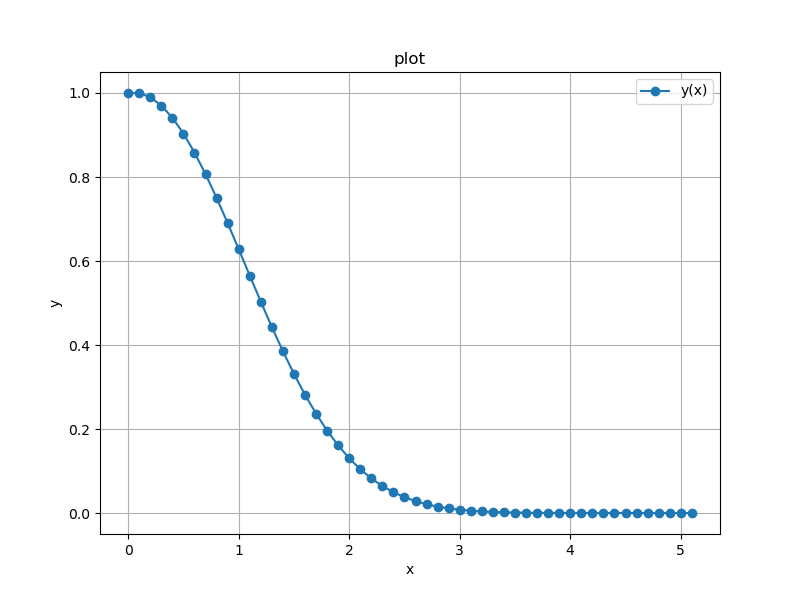
\includegraphics[width=1\columnwidth]{figure/fig.png} 
    \caption{plot}
    \label{stemplot}
 \end{figure}

\end{document}

